% The NYC School System
% Compile with: latexmk -pdf nyc_school_system.tex
\documentclass[aspectratio=169,11pt]{beamer}

\usepackage[T1]{fontenc}
\usepackage{lmodern}
\usepackage{booktabs}
\usepackage{array}
\usepackage{tikz}
\usetikzlibrary{shapes.geometric,positioning,calc,arrows.meta}
\usepackage{pgfplots}
\pgfplotsset{compat=1.18}
\usepackage[most]{tcolorbox}
\graphicspath{{images/}}

% ---------- Colors ----------
\definecolor{navy}{HTML}{1C2541}
\definecolor{oldred}{HTML}{B22234}   % US flag red, also the accent color
\definecolor{oldblue}{HTML}{3C3B6E}  % US flag blue
\definecolor{ink}{HTML}{2B2B2B}
\definecolor{muted}{HTML}{8A8F98}
\definecolor{paper}{HTML}{FFFFFF}
\definecolor{dem}{HTML}{2E5FA3}      % Democrats
\definecolor{rep}{HTML}{C0392B}      % Republicans
\definecolor{austria}{HTML}{C8102E}  % Austria red, for USA-vs-Austria comparisons

% ---------- Minimal theme ----------
\setbeamertemplate{navigation symbols}{}
\setbeamercolor{normal text}{fg=ink, bg=paper}
\setbeamercolor{structure}{fg=navy}
\setbeamercolor{frametitle}{fg=navy}
\setbeamercolor{alerted text}{fg=oldred}
\setbeamercolor{footnote}{fg=muted}
\setbeamerfont{frametitle}{size=\Large, series=\bfseries}
\setbeamertemplate{itemize item}{\color{oldred}\textbullet}
\setbeamertemplate{itemize subitem}{\color{muted}--}
\setbeamertemplate{enumerate item}{\color{oldred}\insertenumlabel.}
\setbeamersize{text margin left=1.1cm, text margin right=1.1cm}
\hypersetup{colorlinks=true, urlcolor=dem, linkcolor=navy}

\setbeamertemplate{frametitle}{%
  \vspace*{0.5cm}%
  \usebeamerfont{frametitle}\usebeamercolor[fg]{frametitle}\insertframetitle\par
  \vspace{0.15cm}{\color{navy!15}\rule{\textwidth}{0.4pt}}\par}

\setbeamertemplate{footline}{%
  \hfill{\tiny\color{muted}\insertframenumber}\hspace*{0.6cm}\vspace*{0.35cm}}

% Plain divider at the start of each section
\AtBeginSection{%
  \begin{frame}[plain,noframenumbering]
    \centering
    {\LARGE\bfseries\color{navy}\insertsection}\\[0.6em]
    {\color{oldred}\rule{1.5cm}{0.8pt}}
  \end{frame}}

% "Think" question slides: \begin{thinkframe} ... \end{thinkframe}
\newenvironment{thinkframe}{%
  \begin{frame}[plain,noframenumbering,environment=thinkframe]\centering\Large}{\end{frame}}

% ---------- Helpers ----------
% Small grey source line at the bottom of a frame
\newcommand{\source}[1]{%
  \begin{tikzpicture}[remember picture,overlay]
    \node[anchor=south west, font=\tiny, text=muted, text width=0.85\paperwidth, align=left]
      at ($(current page.south west)+(0.6cm,0.25cm)$) {#1};
  \end{tikzpicture}}

% US flag drawn in TikZ (hoist height = #1), e.g. \usflag{3cm}
\newcommand{\usflag}[1]{%
  \begin{tikzpicture}[x=#1, y=#1]
    \def\fly{1.9}
    \foreach \i in {0,...,12} {
      \pgfmathsetmacro{\c}{mod(\i,2)==0 ? 1 : 0}
      \ifdim\c pt=1pt
        \fill[oldred] (0,{1-(\i+1)/13}) rectangle (\fly,{1-\i/13});
      \else
        \fill[white] (0,{1-(\i+1)/13}) rectangle (\fly,{1-\i/13});
      \fi
    }
    \def\cw{0.76} \def\ch{0.5385}
    \fill[oldblue] (0,{1-\ch}) rectangle (\cw,1);
    \foreach \r in {1,...,9} {
      \pgfmathsetmacro{\isodd}{mod(\r,2)}
      \ifdim\isodd pt=1pt
        \foreach \k in {0,...,5}
          \node[star, star points=5, star point ratio=2.618, fill=white, inner sep=0pt,
                minimum size=0.0616*#1] at ({(2*\k+1)*\cw/12},{1-\r*\ch/10}) {};
      \else
        \foreach \k in {0,...,4}
          \node[star, star points=5, star point ratio=2.618, fill=white, inner sep=0pt,
                minimum size=0.0616*#1] at ({(2*\k+2)*\cw/12},{1-\r*\ch/10}) {};
      \fi
    }
    \draw[ink!30, line width=0.3pt] (0,0) rectangle (\fly,1);
  \end{tikzpicture}}

% School photo with a letter (and optional name) underneath: \school{file}{width}{label}
\newcommand{\school}[3]{%
  \begin{minipage}[t]{#2}\centering
    \includegraphics[width=\linewidth]{#1}\\[0.2em]
    {\small\bfseries\color{navy}#3}
  \end{minipage}}

% Link box for videos and websites: \linkbox{label}{url}{title}
\newcommand{\linkbox}[3]{%
  \begin{tcolorbox}[enhanced, center, frame hidden, sharp corners, colback=navy!4,
      borderline west={2pt}{0pt}{oldred}, left=10pt, top=8pt, bottom=8pt, width=0.8\textwidth]
    {\small\color{muted}#1}\\[0.2em]
    {\large\href{#2}{#3}}
  \end{tcolorbox}}

% SHSAT question slide: \shsatq{number}{subject}{guide page}{which question}{answer}{explanation}
\newcommand{\guideurl}{https://pwsblobprd.schools.nyc/prd-pws/docs/default-source/default-document-library/nyc-guide-to-the-shsat-for-2027-admissions.pdf}
\newcommand{\shsatq}[6]{%
  \begin{frame}[t]{Question #1 of 5: #2}
    \vspace*{0.3cm}
    \begin{center}
      {\large Open the official guide on \textbf{page #3}:}\\[0.4em]
      {\Large\bfseries\color{navy}#4}\\[1em]
      {\small\href{\guideurl\##3}{NYC Guide to the SHSAT for 2027 Admissions, p.~#3}}\\[1.6em]
      \only<1>{{\large\color{muted}Write down your group's answer!}}%
      \only<2>{{\fontsize{30}{34}\selectfont\bfseries\color{oldred}#5}\\[0.5em]
               {\small #6}}
    \end{center}
    \source{Source: NYC Public Schools / Pearson, \emph{NYC Guide to the SHSAT for 2027 Admissions} (2026).}
  \end{frame}}

\title{The NYC School System}
\author{}
\date{}

\begin{document}

% ---------- Title slide ----------
\begin{frame}[plain]
  \begin{columns}[c]
    \begin{column}{0.55\textwidth}
      {\fontsize{30}{34}\selectfont\bfseries\color{navy} The NYC\\School System}\\[0.8em]
      {\Large\color{muted} Applying to school,\\starting at age 4}\\[0.6em]
      {\color{oldred}\rule{3cm}{1.5pt}}
    \end{column}
    \begin{column}{0.4\textwidth}
      \centering\usflag{2.9cm}
    \end{column}
  \end{columns}
\end{frame}

% =====================================================================
\section{Warm-up}

\begin{frame}{Where are these schools?}
  \centering
  \school{packer.jpg}{0.22\textwidth}{A}\hspace{0.05\textwidth}%
  \school{nightingale.jpg}{0.22\textwidth}{B}\hspace{0.05\textwidth}%
  \school{trinity.jpg}{0.22\textwidth}{C}\\[0.5em]
  \school{stuy.jpg}{0.22\textwidth}{D}\hspace{0.05\textwidth}%
  \school{bxsci.jpg}{0.22\textwidth}{E}\\[0.4em]
  {\large Which of these are actually in \alert{New York}? Why do you think so?}
\end{frame}

\begin{frame}{They're all in New York City}
  \centering
  \school{packer.jpg}{0.185\textwidth}{\footnotesize Packer Collegiate}\hfill
  \school{nightingale.jpg}{0.185\textwidth}{\footnotesize Nightingale-Bamford}\hfill
  \school{trinity.jpg}{0.185\textwidth}{\footnotesize Trinity School}\hfill
  \school{stuy.jpg}{0.185\textwidth}{\footnotesize Stuyvesant}\hfill
  \school{bxsci.jpg}{0.185\textwidth}{\footnotesize Bronx Science}\\[0.8em]
  \raggedright
  \begin{itemize}\setlength{\itemsep}{0.5em}
    \item \textbf{A, B, C:} \alert{private} schools. Tuition: about \textbf{\$69,000 a year} (Trinity, 2025--26)
    \item \textbf{D, E:} \alert{public} schools. Tuition: \textbf{\$0}, but you need a top score on an entrance exam
    \item In 2026--27, at least \textbf{seven} NYC private schools charge more than \textbf{\$70,000 a year}
  \end{itemize}
  \source{Sources: Fortune, Feb.\ 2025; Bloomberg, Feb.\ 2026. Photos: Ajay Suresh, CC BY 2.0 (Packer, Nightingale-Bamford); Jay Dobkin, CC BY-SA 4.0 (Trinity); Kidfly182, CC BY-SA 4.0 (Stuyvesant); Bxsstudent, public domain (Bronx Science). All via Wikimedia Commons.}
\end{frame}

% =====================================================================
\section{Basic Info}

\begin{frame}{NYC schools by the numbers}
  \begin{itemize}\setlength{\itemsep}{0.7em}
    \item \textbf{About 885,000} students in NYC Public Schools (3-K to 12th grade, 2025--26)
    \item \textbf{Plus about 151,000} in public \alert{charter} schools (publicly funded, privately run)
    \item \textbf{1,599} schools run by NYC Public Schools
    \item \textbf{Roughly 200,000} in \alert{private} schools, most of them religious (Jewish and Catholic)
    \item About \textbf{73\%} of public school students live in poverty; \textbf{14\%} are homeless or in temporary housing
  \end{itemize}
  \source{Sources: NYC Public Schools, \emph{Data at a Glance} (2025--26); NYC Comptroller, \emph{Tracking the K-12 Student Population in NYC} (Oct.\ 2026).}
\end{frame}

\begin{frame}{One city, one country}
  \vfill
  \centering
  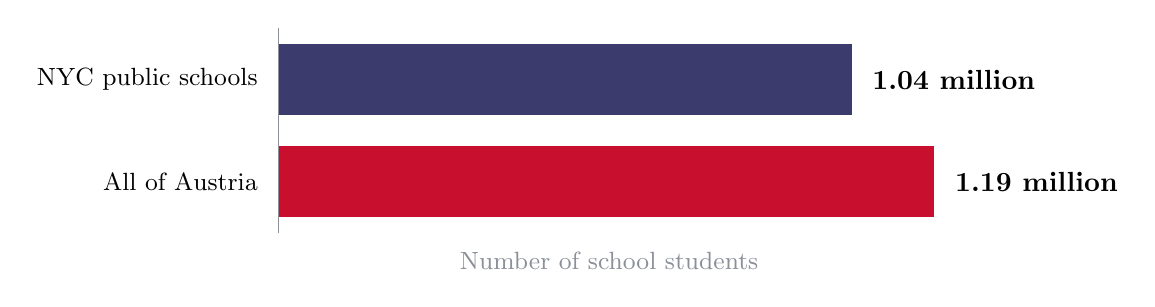
\begin{tikzpicture}[x=7cm, y=-1cm]
    \foreach \y/\lab/\v/\txt/\col in {0/{NYC public schools}/1.04/{1.04 million}/oldblue,
                                      1.3/{All of Austria}/1.19/{1.19 million}/austria} {
      \fill[\col] (0,\y) rectangle (\v,\y+0.9);
      \node[anchor=east, font=\small, align=right] at (-0.02,\y+0.45) {\lab};
      \node[anchor=west, font=\bfseries] at (\v+0.02,\y+0.45) {\txt};
    }
    \draw[muted] (0,-0.2) -- (0,2.4);
    \node[font=\small, text=muted] at (0.6,2.75) {Number of school students};
  \end{tikzpicture}
  \vfill
  {\large NYC's public schools are almost as big as \alert{Austria's entire school system}.}
  \vfill
  \source{Sources: NYC Public Schools (2025--26, district + charter schools); Statistik Austria via ORF (2024/25: 1,185,525 students).}
\end{frame}

\begin{frame}{The basic structure}
  \centering
  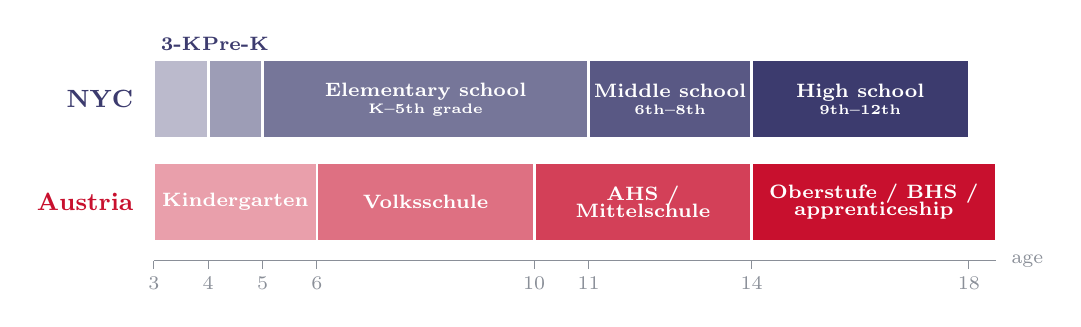
\begin{tikzpicture}[x=0.69cm, y=1cm]
    % NYC row
    \foreach \a/\b/\lab/\shade in {3/4/{}/35, 4/5/{}/50,
                                  5/11/{Elementary school\\[-0.2em]{\tiny K--5th grade}}/70,
                                  11/14/{Middle school\\[-0.2em]{\tiny 6th--8th}}/85,
                                  14/18/{High school\\[-0.2em]{\tiny 9th--12th}}/100} {
      \fill[oldblue!\shade, draw=white, line width=1pt] (\a,1.3) rectangle (\b,2.3);
      \node[text=white, font=\scriptsize\bfseries, align=center] at ({(\a+\b)/2},1.8) {\lab};
    }
    % Austria row
    \foreach \a/\b/\lab/\shade in {3/6/{Kindergarten}/40,
                                  6/10/{Volksschule}/60,
                                  10/14/{AHS /\\[-0.2em]Mittelschule}/80,
                                  14/18.5/{Oberstufe / BHS /\\[-0.2em]apprenticeship}/100} {
      \fill[austria!\shade, draw=white, line width=1pt] (\a,0) rectangle (\b,1);
      \node[text=white, font=\scriptsize\bfseries, align=center] at ({(\a+\b)/2},0.5) {\lab};
    }
    \node[anchor=east, font=\small\bfseries, text=oldblue] at (2.8,1.8) {NYC};
    \node[font=\scriptsize\bfseries, text=oldblue, anchor=south] at (3.5,2.3) {3-K};
    \node[font=\scriptsize\bfseries, text=oldblue, anchor=south] at (4.5,2.3) {Pre-K};
    \node[anchor=east, font=\small\bfseries, text=austria] at (2.8,0.5) {Austria};
    % Age axis
    \draw[muted] (3,-0.25) -- (18.5,-0.25);
    \foreach \x in {3,4,5,6,10,11,14,18} {
      \draw[muted] (\x,-0.25) -- (\x,-0.35);
      \node[font=\scriptsize, text=muted, below] at (\x,-0.33) {\x};
    }
    \node[font=\scriptsize, text=muted, anchor=west] at (18.6,-0.25) {age};
  \end{tikzpicture}

  \vspace{1.2em}
  \raggedright
  \begin{itemize}
    \item In NYC, 3-K and Pre-K are \alert{free}, but not compulsory
  \end{itemize}
\end{frame}

% =====================================================================
\section{The Path to College}

\begin{frame}{Remember: getting into college}
  \vfill
  \centering
  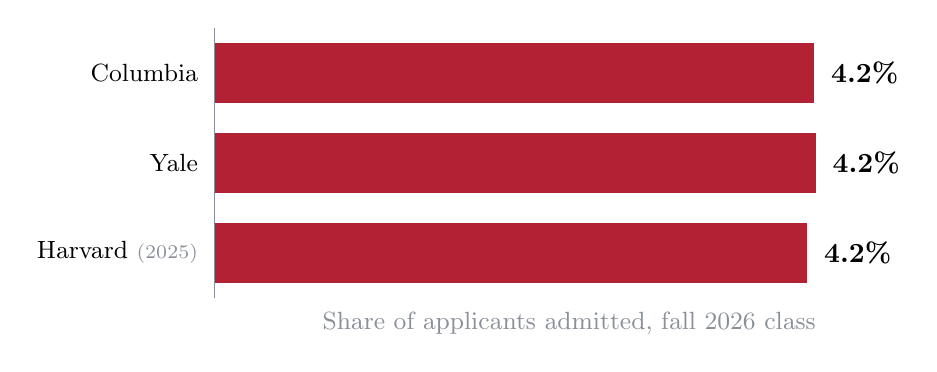
\begin{tikzpicture}[x=1.8cm, y=-0.95cm]
    \foreach \y/\lab/\v/\txt in {0/{Columbia}/4.23/{4.2\%},
                                 1.2/{Yale}/4.24/{4.2\%},
                                 2.4/{Harvard {\scriptsize\color{muted}(2025)}}/4.18/{4.2\%}} {
      \fill[oldred] (0,\y) rectangle (\v,\y+0.8);
      \node[anchor=east, font=\small] at (-0.05,\y+0.4) {\lab};
      \node[anchor=west, font=\bfseries] at (\v+0.05,\y+0.4) {\txt};
    }
    \draw[muted] (0,-0.2) -- (0,3.4);
    \node[font=\small, text=muted] at (2.5,3.75) {Share of applicants admitted, fall 2026 class};
  \end{tikzpicture}
  \vfill
  {\large Fewer than \alert{1 in 20} applicants get in.}
  \vfill
  \source{Sources: Yale News, Mar.\ 2026 (2,328 of 54,919); Columbia via \emph{Columbia Spectator} (2,581 of 61,031); \emph{Harvard Crimson}, Oct.\ 2025 (Class of 2029: 2,003 of 47,893).}
\end{frame}

\begin{frame}{But\ldots}
  \begin{itemize}\setlength{\itemsep}{0.9em}
    \item Most American colleges admit \alert{most} students who apply
    \item More than half of four-year colleges accept \textbf{two-thirds} or more of applicants
    \item Only \textbf{17} of about 1,364 four-year colleges accepted fewer than \textbf{10\%}
    \item The pressure is about getting into the \alert{top} schools, and in NYC that race starts early
  \end{itemize}
  \source{Source: Pew Research Center, 2019 (data for 2017).}
\end{frame}

\begin{frame}[plain]
  \vfill
  \begin{center}
    {\LARGE\bfseries For NYC students, the application\\process begins in \alert{pre-K}.}
  \end{center}
  \vfill
\end{frame}

\begin{frame}{Applying to elementary school}
  \begin{itemize}\setlength{\itemsep}{0.6em}
    \item Every 5-year-old in NYC is \alert{guaranteed} a kindergarten seat, but not at a specific school
    \item Families rank schools; if a school has more applicants than seats, there's a \alert{lottery}
    \item Who gets priority (in order):
  \end{itemize}
  \vspace{0.2em}
  \begin{enumerate}\setlength{\itemsep}{0.25em}\leftskip=1.2em
    \item Live in the school's \textbf{zone} and have a \textbf{sibling} there
    \item Live in the school's \textbf{zone}
    \item Have a \textbf{sibling} at the school (but live outside the zone)
    \item Attend the school's \textbf{pre-K}
  \end{enumerate}
  \source{Source: NYC Public Schools, kindergarten admissions (fall 2027 cycle).}
\end{frame}

\begin{frame}{Gifted and Talented (G\&T)}
  \begin{itemize}\setlength{\itemsep}{0.45em}
    \item Separate, accelerated classes, starting in \alert{kindergarten}
    \item About \textbf{2,500} kindergarten seats a year; about 18,000 G\&T students in total
    \item How do 4-year-olds get in?
      \begin{itemize}
        \item Public pre-K students: their \textbf{pre-K teacher} evaluates them
        \item Private pre-K or no pre-K: an \textbf{interview} with the Education Department
        \item Eligible children then enter a \textbf{lottery}
      \end{itemize}
    \item Until 2021, children took a \alert{test} at age 4
    \item \textbf{Mayor Mamdani} wants to stop admitting kindergartners to G\&T; for now the program continues (fall 2027 applications open Dec.\ 2026)
  \end{itemize}
  \source{Sources: NYC Public Schools, Gifted and Talented; AP and news reports, 2025--26.}
\end{frame}

\begin{frame}{Elementary school}
  \begin{itemize}\setlength{\itemsep}{0.9em}
    \item School day: about \textbf{8:30 a.m. to 3:00 p.m.} {\small\color{muted}(6 hours 20 minutes; times vary by school)}
    \item One main teacher, one classroom, the same classmates all day
    \item Subjects: Math, English Language Arts (ELA), Science, Social Studies, Spanish, Music, Technology
    \item After \textbf{5th grade} (age 10--11): you must \alert{apply} to middle school
  \end{itemize}
  \source{Source: Chalkbeat, Apr.\ 2026 (length of the school day).}
\end{frame}

\begin{frame}{Applying to middle school}
  \begin{itemize}\setlength{\itemsep}{0.7em}
    \item Apply in the fall of 5th grade and rank schools in order of preference
    \item Some schools use a \alert{lottery} with priorities (e.g.\ living in the district)
    \item Others \alert{screen} students using \textbf{4th-grade report card grades}
    \item This is when many families \textbf{leave} the public schools: the biggest drop in enrollment happens between 5th and 6th grade
    \item Example: my middle school, \textbf{MS 54 Booker T.\ Washington} (Upper West Side): \href{https://www.ms54.org/admissions}{ms54.org/admissions}
  \end{itemize}
  \source{Sources: NYC Public Schools, middle school admissions; NYC Comptroller, Oct.\ 2026.}
\end{frame}

\begin{frame}{Watch: a school tour}
  \vfill
  \centering
  \linkbox{Watch:}{https://www.youtube.com/results?search_query=Elster+school+tour}{Elster school tour}
  \vfill
\end{frame}

% =====================================================================
\section{Applying to High School}

\begin{frame}{Three separate applications}
  \begin{itemize}\setlength{\itemsep}{0.45em}\small
    \item \textbf{1. Specialized High Schools} (8 schools): admission by \alert{one test only}, the SHSAT
      \begin{itemize}
        \item e.g.\ Stuyvesant, Bronx Science, Brooklyn Tech
      \end{itemize}
    \item \textbf{2. LaGuardia High School} (performing and visual arts): admission by \alert{audition} or portfolio
    \item \textbf{3. The main application:} 700+ programs at 400+ high schools
      \begin{itemize}
        \item \textbf{Screened} programs: grades, attendance, sometimes interviews
        \item \textbf{Audition} programs, e.g.\ Frank Sinatra School of the Arts
        \item \textbf{Open} programs: lottery
      \end{itemize}
    \item Each application can give you \alert{at most one offer}
  \end{itemize}
  \source{Source: NYC Public Schools, high school admissions.}
\end{frame}

\begin{frame}{Happening right now}
  \begin{itemize}\setlength{\itemsep}{0.9em}
    \item This month, about \textbf{26,000} NYC 8th graders take the \alert{SHSAT}
      \begin{itemize}
        \item Test days: \textbf{Nov.\ 14/15 and 21, 2026}
      \end{itemize}
    \item High school applications are due \textbf{Dec.\ 4, 2026}
    \item Offers arrive \textbf{March 3, 2027}
  \end{itemize}
  \source{Source: NYC Public Schools, fall 2027 admissions calendar.}
\end{frame}

\begin{frame}{The SHSAT}
  \begin{itemize}\setlength{\itemsep}{0.7em}
    \item \textbf{3 hours}, \textbf{100 questions} (50 English, 50 Math), no calculator
    \item New in 2026: taken on a \alert{computer}, and \alert{adaptive}: get a question right and the next one is harder
    \item \alert{Your score is the only thing that counts.} No grades, no interviews, no essays
    \item About \textbf{26,100} students took it last year; about \textbf{4,000} got an offer (about \textbf{1 in 6})
    \item Lowest score that got into Stuyvesant: \textbf{561} (2026 admissions)
  \end{itemize}
  \source{Sources: NYC Public Schools, \emph{NYC Guide to the SHSAT for 2027 Admissions}; Chalkbeat, July 2026.}
\end{frame}

\begin{frame}{Who gets in?}
  \begin{columns}[c]
    \begin{column}{0.44\textwidth}
      \centering
      {\small\color{muted} Share of offers to the eight test schools, fall 2026\par}
      \vspace{0.6em}
      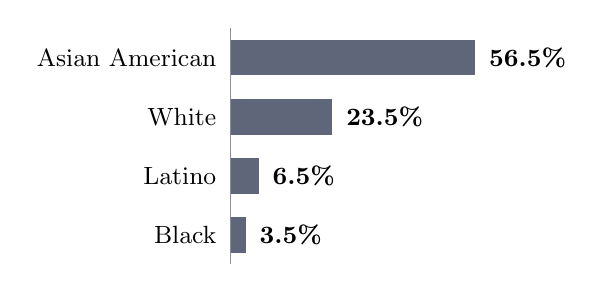
\begin{tikzpicture}[x=0.055cm, y=-0.75cm]
        \foreach \y/\lab/\v in {0/{Asian American}/56.5, 1/White/23.5, 2/Latino/6.5, 3/Black/3.5} {
          \fill[navy!70] (0,\y) rectangle (\v,\y+0.6);
          \node[anchor=east, font=\small] at (-1,\y+0.3) {\lab};
          \node[anchor=west, font=\small\bfseries] at (\v+1,\y+0.3) {\v\%};
        }
        \draw[muted] (0,-0.2) -- (0,3.8);
      \end{tikzpicture}
    \end{column}
    \begin{column}{0.5\textwidth}
      \begin{itemize}\setlength{\itemsep}{0.6em}\small
        \item Stuyvesant offered seats to \textbf{3} Black students
        \item \textbf{Supporters} of the test: it's \alert{objective}, the same rules for everyone
        \item \textbf{Critics}: it favors families who can pay for \alert{test prep} and leaves out Black and Latino students
        \item Mayor Mamdani has said he will \textbf{keep} the test and study it for bias
      \end{itemize}
    \end{column}
  \end{columns}
  \source{Source: Chalkbeat, July 2026.}
\end{frame}

\begin{frame}{No guarantee}
  \begin{itemize}\setlength{\itemsep}{0.7em}
    \item Applying to all three is \alert{far from a guarantee}
    \item At my middle school, about \textbf{30 students} got \textbf{no} high school offer at all in the first round
    \item There's usually \alert{no ``default'' school}: most NYC high schools aren't zoned
    \item Students without an offer go on \textbf{waitlists} and are placed later at a school with open seats
    \item Citywide (2024): about \textbf{3\%} of applicants got no offer to any school on their list
  \end{itemize}
  \source{Source: NYC Public Schools, 2024 admissions cycle data release.}
\end{frame}

\begin{frame}{What does high school look like?}
  \begin{itemize}\setlength{\itemsep}{0.9em}
    \item \alert{Highly dependent on which school you go to}
    \item Some schools have \textbf{thousands} of students; others fewer than \textbf{150}
    \item Specialized schools: very competitive, lots of homework, many AP courses
    \item Small schools: themes like law, health, technology, or the arts
  \end{itemize}
\end{frame}

\begin{frame}{My high school}
  \begin{itemize}\setlength{\itemsep}{0.9em}
    \item About \textbf{150 students per grade}
    \item An \alert{``Early College''} program: college courses during high school, for free college credit
    \item A \textbf{5-story} building
  \end{itemize}
  \vspace{1em}
  \centering
  \linkbox{Take a look:}{https://www.google.com/maps}{Google Street View}
\end{frame}

\begin{frame}{My schedule}
  \vfill
  \centering
  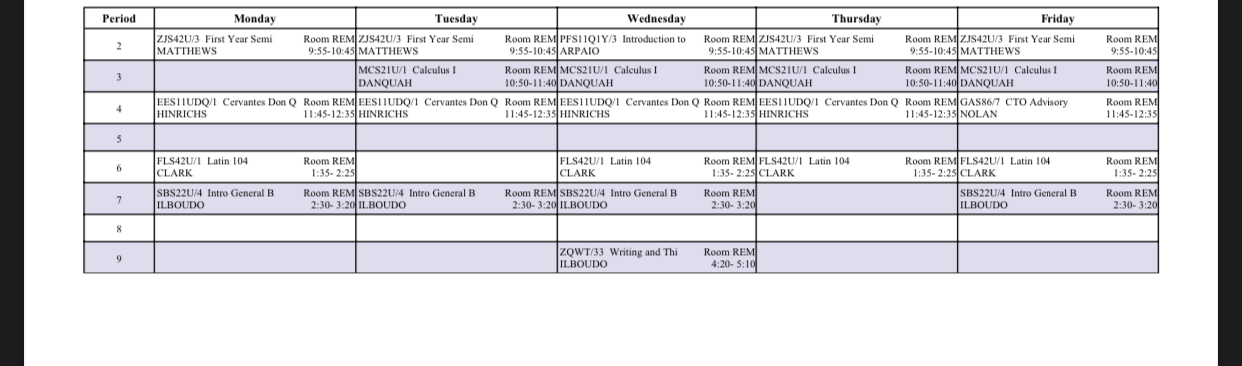
\includegraphics[width=\textwidth, trim={28bp 28.5bp 26.7bp 0bp}, clip]{schedule.jpg}\\[1em]
  \raggedright
  {\small College-level courses: \alert{Calculus I}, \alert{Latin}, \alert{Intro to General Biology}, \alert{Cervantes' \emph{Don Quixote}}\par}
  \vfill
\end{frame}

\begin{frame}{Next step: college}
  \begin{itemize}\setlength{\itemsep}{0.8em}
    \item At my school, getting A's was \alert{relatively easy}
    \item So: ``spam'' extracurriculars, i.e.\ do as many as you can
    \item Popular activities at my school:
      \begin{itemize}\setlength{\itemsep}{0.3em}
        \item \textbf{Clubs:} Quiz Bowl, Model UN, Debate
        \item \textbf{Sports:} Frisbee, Tennis
      \end{itemize}
  \end{itemize}
\end{frame}

% =====================================================================
\section{Compare}

\begin{frame}{Sorting students: NYC vs.\ Austria}
  \footnotesize
  \renewcommand{\arraystretch}{1.25}
  \begin{tabular}{@{}>{\raggedright\arraybackslash}p{0.17\textwidth}>{\raggedright\arraybackslash}p{0.39\textwidth}>{\raggedright\arraybackslash}p{0.39\textwidth}@{}}
    \toprule
    & \textbf{\color{oldblue}NYC} & \textbf{\color{austria}Austria} \\
    \midrule
    First selection & G\&T at \textbf{4--5} & Gymnasium (AHS) or Mittelschule at \textbf{10} \\
    Middle school & Apply at \textbf{10--11} (lottery or grades) & Based on Volksschule grades \\
    High school & Apply at \textbf{13--14}; one test for the top 8 schools & Oberstufe, BHS (HTL, HAK \ldots) or apprenticeship at \textbf{14} \\
    Private schools & Many, up to \textbf{\$70,000+} a year & Mostly Catholic, far cheaper \\
    University & Applications, essays, tests; under 5\% at top schools & Matura, then mostly \textbf{open} admission; free for EU students (within standard study time) \\
    \bottomrule
  \end{tabular}
  \source{Sources: NYC Public Schools; oesterreich.gv.at; studium.at.}
\end{frame}

\begin{thinkframe}
  {\color{oldred}\textbf{Think}}\\[0.8em]
  Austria is often criticized for sorting kids at 10.\\
  Is New York better or worse?
\end{thinkframe}

% =====================================================================
\section{Final Activity}

\begin{frame}{Could you get into Stuyvesant?}
  \begin{itemize}\setlength{\itemsep}{0.9em}
    \item In your groups: answer \textbf{5 real questions} from the official SHSAT guide
    \item \alert{No calculators!}
    \item Write down your answers; we'll check them after each question
    \item Real 8th graders get less than \textbf{2 minutes} per question
  \end{itemize}
\end{frame}

\shsatq{1}{Math}{23}{The marbles question\\{\normalsize\mdseries (Jenny and Keiko)}}{D) 40}{Jenny has $J = 2K$ marbles; after giving 5: $J-5 = (K+5)+10$, so $J = 40$.}

\shsatq{2}{Math}{24}{The rectangle question\\{\normalsize\mdseries (perimeter 510 cm, ratio 3:2)}}{F) 153 cm by 102 cm}{Sides $3x$ and $2x$: $10x = 510$, so $x = 51$.}

\shsatq{3}{Math}{25}{The ``lorgs and dalts'' question\\{\normalsize\mdseries (exchanging money)}}{B) \$52}{140 lorgs $= \$20$ and 16 dalts $= \$32$.}

\shsatq{4}{English}{17}{The Yankees paragraph\\{\normalsize\mdseries (a shift in verb tense)}}{A) Sentence 1}{``meant'' should be ``means'' or ``will mean.''}

\shsatq{5}{English}{18}{The Airbnb paragraph\\{\normalsize\mdseries (an error in construction)}}{F) Sentence 2}{The opening phrase should describe the roommates, not the air mattresses.}

\begin{frame}{How did you do?}
  \begin{itemize}\setlength{\itemsep}{1em}
    \item Which group got the most right?
    \item Which section was harder for you: \alert{English} or \alert{Math}? Why?
    \item Should one test decide who gets into the best public high schools?
  \end{itemize}
\end{frame}

\end{document}
